\documentclass[12pt, a4paper, twoside]{article}
\usepackage[utf8]{inputenc}
\usepackage[cm]{fullpage}
\usepackage{fancyhdr}
\usepackage{textcomp}
\usepackage{graphicx}
\usepackage{commath}
\usepackage[portuguese]{babel}

\begin{document}

\title{Pré-relatório 1 do Laboratório de Dispositivos e Circuitos Eletrônicos}
\author{Cristiano Silva Júnior: 13/0070629}
\date{\today}
\maketitle

Neste pré-relatório, consideraremos um amplificador operacional (\textit{amp op}) ideal como o do modelo da figura 1.

\begin{figure}
    \centering
    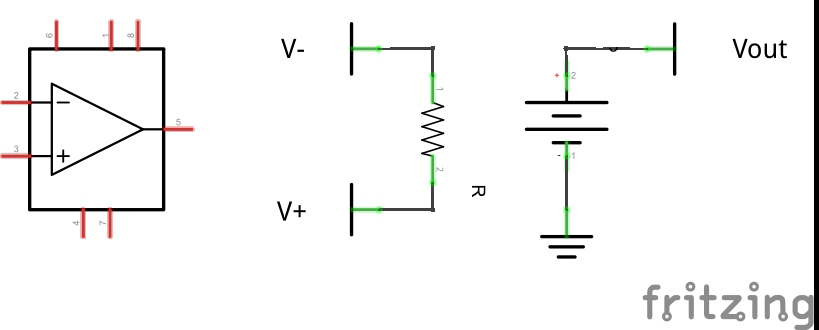
\includegraphics[width=0.8\textwidth]{figs/ex0.jpg}
    \caption{Modelo do amplificador operacional}
\end{figure}

Consideramos, neste modelo, que
$$ V_{out} = A (V_+ - V_-) $$
e que tanto
$$ R = \infty $$
como
$$ A = \infty $$

\section{Exercício 1}

Utilizando o amplificador operacional \textit{LM741} da \textit{National Instruments} como referência, extraí os seguintes valores para os parâmetros requisitados:

\begin{itemize}
    \item Corrente de compensação de entrada (input offset current): $20nA$ típico, $200nA$ máximo.
    \item Tensão de compensação de entrada (input offset voltage): $1mV$ típico, $5mV$ máximo.
    \item Corrente de polarização de entrada (input bias current): $80nA$ típico, $500nA$ máximo.
    \item Resistência de entrada (input resistance): $2M\Omega$ típico, $0.3M\Omega$ mínimo.
    \item Razão de rejeição em modo comum (CMRR - Common-Mode Rejection ratio): $95dB$ típico, $80dB$ mínimo.
    \item Largura de banda (bandwidth): $1.5MHz$ típico, $0.437MHz$ mínimo.
    \item Taxa de variação (slew rate): $0.7V/\mu s$ típico, $0.3V/\mu s$ mínimo.
    \item Potência consumida: $50mW$ típico, $85mW$ máximo.
    \item Corrente de saída em curto-circuito (output short circuit current): $25mA$ típico.
    \item Razão de rejeição da fonte de alimentação (PSRR – power supply voltage rejection ratio): $96dB$ típico, $86dB$ mínimo.
\end{itemize}

Segundo o fabricante, estes valores foram coletados em um experimento a $25^oC$ de temperatura ambiente.

\section{Exercício 2}

Diz-se que a média entre as entradas de qualquer dispositivo é um sinal de modo comum ($v_c$). No caso do amplificador operacional, $v_c := \frac{v_+ + v_-}{2}$. Associado a este número, temos também a diferença entre as entradas $v_d := v_+ - v_-$.

A partir disso, podemos definir o ganho em modo comum $A_c$ e o ganho em modo diferencial $A_d$. Estes ganhos são as parcelas de cada um dos sinal de entrada que contribuem para o ganho total do amplificador. Com base nesta intuição, a saída do \textit{amp op} pode ser reescrita como sendo $v_o = v_c A_c + v_d A_d$.

É interessante definir estas grandezas pois um dos parâmetros que são levados em consideração na hora de construir um \textit{opamp} é a razãode rejeição em modo comum $CMRR$. Este valor é constante e diz o quão bom o dispositivo é para subtrair os sinais de entrada. É dado por $CMRR = 20 log_{10} \abs{\frac{A_d}{A_c}} $

\section{Exercício 3}

No modelo do \textit{amp op}, temos que, entre as entradas, há um resistor, cuja diferença de tensão determinará qual a tensão de saída do dispositivo. Idealmente, a resistência de entrada é infinita. Se ela é infinita, a corrente que passa por este resistor é nula. Se a corrente é nula, então entende-se que não diferença de tensão entre os pontos. Desta forma, a tensão entre os terminais do \textit{amp op} deverá ser a mesma, o que é equivalente a dizer que há um curto circuito naquela região do circuito. Como este curto não existe, já que há um resistor ali, dizemos que este é um curto circuito virtual.

\section{Exercício 4}

\begin{figure}
    \centering
    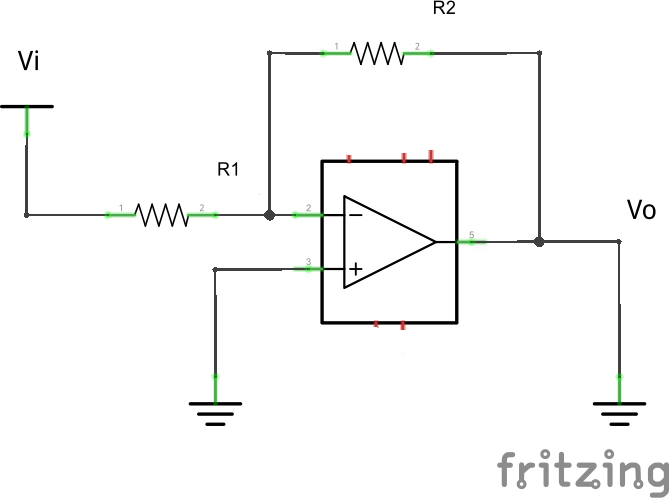
\includegraphics[width=0.8\textwidth]{figs/ex4.jpg}
    \caption{Circuito analisado no problema 4}
\end{figure}

Supondo o \textit{amp op} do exercício como ideal, temos que a corrente que entra no dispositivo é nula, e que a tensão em $v = 0$. Pela lei de Kirchhoff das correntes,
$$  i_1 = i_2 $$
$$ \Rightarrow \frac{v_i - v}{R_1} = \frac{v - v_o}{R_2} $$
$$ \Rightarrow \frac{v_o}{v_i} = -\frac{R_2}{R_1} $$

Sendo assim, podemos concluir que

$$ i_1 = \frac{v_1}{R_1} $$
$$ i_2 = -\frac{v_o}{R_2} $$

\section{Exercício 5}

O circuito da figura (a) do roteiro pode ser resolvido por um simples divisor de tensão, resultando em $\frac{5}{11}V$.

O circuito do figura (c) do roteiro requer que descubramos a função de transferência do circuito na figura 3.

\begin{figure}
    \centering
    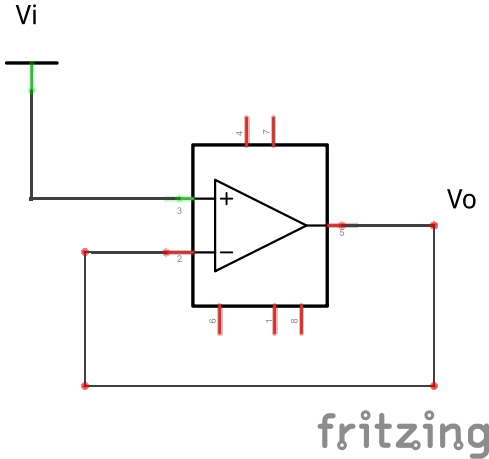
\includegraphics[width=0.8\textwidth]{figs/ex5.jpg}
    \caption{Seguidor de tensão}
\end{figure}

Este é o seguidor de tensão, e sua principal característica é que $v_i = v_o$.

Como não há corrente de entrada no \textit{amp op}, então a tensão que entra no dispositivo é $5V$, já que não haverá queda de tensão no resistor de $10k\omega$. Portanto, a tensão sobre o resistor de $1k\omega$ será de $5V$

\section{Exercício 6}

O \textit{slew rate} é a maior derivada com relação ao tempo que a tensão de saída um dispositivo pode assumir. Depois

A diferença de tensão que anula a saida de um \textit{amp op} é definida como tensão de compensação de entrada.

A diferença absoluta entre as correntes de fuga da entrada inversora e da não-inversora é denominada corrente de compensação de entrada. A média entre essas correntes de fuga é chamada de corrente de polarização.

\section{Exercício 7}

Considerando o efeito do \textit{slew rate} (SR), espera-se que a saída do circuito seja uma rampa que sature em $v_e$ (ou em $12V$ se $v_e$ for maior do que a alimentação).

Considerando que a saída seja $a = 1V$ e o SR do $LM741$ da \textit{National Instruments}, espera-se que o \textit{amp op} sature em aproximadamente $1.43 \mu s$. Desta forma, a rampa quase não deve ser enxergada em situações comuns de uso.

\section{Referência Bibliográfica}

\begin{itemize}
    \item Apostila do professor Humberto. http://paginapessoal.utfpr.edu.br/humberto/atividade-de-ensino/inicio/labeltronica. Acesso em 14 de Agosto de 2017.
    \item \textit{Datasheet} do $LM741$. http://www.ti.com/lit/ds/symlink/lm741.pdf. Acesso em 14 de Agosto de 2017.
\end{itemize}

\end{document}
